% Words Beyond the Rate v10.3 — Conference Presentation
% Beamer 16:9, paper-navbar
\documentclass[aspectratio=169, 11pt]{beamer}

% ── Theme ──
\usetheme{Madrid}
\usecolortheme{whale}
\usefonttheme{professionalfonts}
\usepackage[most]{tcolorbox}
\usepackage{booktabs}
\usepackage{graphicx}
\usepackage{amsmath,amssymb}
\usepackage{tikz}
\usetikzlibrary{arrows.meta, positioning, shapes.geometric}
\usepackage{ragged2e}
\justifying
\usepackage{hyperref}
\hypersetup{hidelinks}
\graphicspath{{figures/}}

% ── Colors ──
\definecolor{myblue}{HTML}{2B5EA7}
\definecolor{myred}{HTML}{C0392B}
\definecolor{mygreen}{HTML}{27AE60}
\definecolor{mygray}{HTML}{F5F5F5}
\definecolor{darkbg}{HTML}{1B2A4A}

% ── tcolorbox styles ──
\tcbset{
  blocksty/.style={
    boxrule=0.4pt, arc=1.5pt,
    top=2pt, bottom=2pt, left=4pt, right=4pt,
    fonttitle=\bfseries\small, before upper={\small}, valign=top,
  }
}
\newtcolorbox{fblock}[2][]{blocksty, colback=myblue!8, colframe=myblue!85,
  coltitle=white, title={#2}, height=#1}
\newtcolorbox{falertblock}[2][]{blocksty, colback=myred!8, colframe=myred!80,
  coltitle=white, title={#2}, height=#1}
\newtcolorbox{ablock}[1]{blocksty, colback=myblue!8, colframe=myblue!85,
  coltitle=white, title={#1}}
\newtcolorbox{aalertblock}[1]{blocksty, colback=myred!8, colframe=myred!80,
  coltitle=white, title={#1}}
\newtcolorbox{aexampleblock}[1]{blocksty, colback=mygreen!8, colframe=mygreen!80,
  coltitle=white, title={#1}}

% ── Navigation ──
\useoutertheme{miniframes}
\input{paper-navbar.tex}

% ── Metadata ──
\title[Words Beyond the Rate]{Words Beyond the Rate: High-Frequency Monetary Policy Shocks and FOMC Language}
\author[Zhang \& Yang]{Eileen Zhang, Dechang Yang}
\date[XJTLU, 2026]{}
\institute{Xi'an Jiaotong-Liverpool University}

\begin{document}

% ============================================================
% TITLE
% ============================================================
\begin{frame}[plain]
\titlepage
\end{frame}

% ============================================================
% OUTLINE
% ============================================================
\begin{frame}{Outline}
\tableofcontents
\end{frame}

% ============================================================
\section{Motivation}
% ============================================================

\begin{frame}{FOMC Language Moves Markets --- Not Just Rates}
\begin{columns}[T]
\column{0.52\textwidth}
\begin{ablock}{The Taper Tantrum (2013)}
\begin{itemize}
  \item FOMC kept rates unchanged
  \item Language shift: ``may reduce'' asset purchases
  \item 10Y Treasury yield rose 40 bp in days
  \item Markets reacted to \textbf{words}, not the rate
\end{itemize}
\end{ablock}
\vspace{0.3em}
\begin{aalertblock}{Core Question}
Does FOMC statement language convey information \textbf{beyond} the rate decision itself?
\end{aalertblock}

\column{0.44\textwidth}
\begin{center}
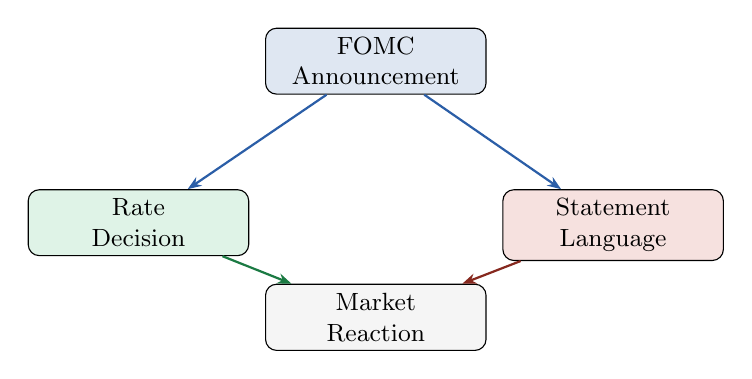
\begin{tikzpicture}[
  box/.style={draw, rounded corners, minimum width=2.8cm, minimum height=0.8cm,
    font=\small, align=center},
  arr/.style={-{Stealth[length=5pt]}, thick}
]
\node[box, fill=myblue!15] (fomc) {FOMC\\Announcement};
\node[box, fill=mygreen!15, below left=1.2cm and 0.2cm of fomc] (rate) {Rate\\Decision};
\node[box, fill=myred!15, below right=1.2cm and 0.2cm of fomc] (lang) {Statement\\Language};
\node[box, fill=mygray, below=2.4cm of fomc] (mkt) {Market\\Reaction};
\draw[arr, myblue] (fomc) -- (rate);
\draw[arr, myblue] (fomc) -- (lang);
\draw[arr, mygreen!70!black] (rate) -- (mkt);
\draw[arr, myred!70!black] (lang) -- (mkt);
\end{tikzpicture}
\par\vspace{0.15em}
{\scriptsize \textbf{Figure 1.} Two channels of FOMC influence}
\end{center}
\end{columns}
\end{frame}

% ============================================================
\begin{frame}{Two Competing Interpretations}
\begin{columns}[T]
\column{0.48\textwidth}
\begin{fblock}[5.5cm]{Policy Implementation}
\begin{itemize}
  \item Statement \textbf{explains} the decision
  \item Target shock drives sentiment
  \item Language reflects \emph{what was done}
  \item Bernanke \& Kuttner (2005)
\end{itemize}
\end{fblock}

\column{0.48\textwidth}
\begin{falertblock}[5.5cm]{Informational Revelation}
\begin{itemize}
  \item Statement \textbf{reveals} future policy intent
  \item Path shock (FG) drives sentiment
  \item Language signals \emph{what will be done}
  \item Romer \& Romer (2000), Campbell et al.\ (2012)
\end{itemize}
\end{falertblock}
\end{columns}

\vspace{0.5em}
\begin{center}
\textbf{Our contribution:} Decompose which channel dominates using GSS high-frequency shocks + textual sentiment analysis
\end{center}
\end{frame}

% ============================================================
\section{Data \& Methodology}
% ============================================================

\begin{frame}{Data Overview: 117 FOMC Meetings (2006--2022)}
\begin{columns}[T]
\column{0.48\textwidth}
\begin{ablock}{Monetary Policy Shocks}
\begin{itemize}
  \item \textbf{Target}: GSS current-rate surprise
  \item \textbf{Path}: GSS future-policy revision
  \item Source: Acosta (2022)
  \item $\rho = 0.14$ (successfully separated)
\end{itemize}
\end{ablock}
\vspace{0.2em}
\begin{aexampleblock}{Sentiment Measures}
\begin{itemize}
  \item LM: Loughran-McDonald
  \item CB: Central-bank-specific
  \item Combined: $0.5 \times \text{LM} + 0.5 \times \text{CB}$
\end{itemize}
\end{aexampleblock}

\column{0.48\textwidth}
\begin{ablock}{Financial Market Data}
\begin{itemize}
  \item CRSP VW/EW/S\&P 500 (WRDS)
  \item NASDAQ, Gold
  \item 10Y Treasury, 13W T-bill
  \item VIX index
\end{itemize}
\end{ablock}
\vspace{0.2em}
\begin{aalertblock}{Key Features}
\begin{itemize}
  \item 3 Chairs: Bernanke, Yellen, Powell
  \item 3 Regimes: conventional, FG, normalization
  \item FG: Dec 2008 -- Dec 2015 (57 meetings)
\end{itemize}
\end{aalertblock}
\end{columns}
\end{frame}

% ============================================================
\begin{frame}{Empirical Framework}
\begin{columns}[T]
\column{0.48\textwidth}
\begin{ablock}{H1: Sentiment $\sim$ Shocks}
\[
S_t = \alpha + \beta_T \cdot \text{Target}_t + \beta_P \cdot \text{Path}_t + \varepsilon_t
\]
\end{ablock}
\vspace{0.2em}
\begin{ablock}{H2: Returns $\sim$ Shocks}
\[
R_t = \alpha + \beta_T \cdot \text{Target}_t + \beta_P \cdot \text{Path}_t + \varepsilon_t
\]
\end{ablock}

\column{0.48\textwidth}
\begin{ablock}{H3: Wald Test ($\beta_T = \beta_P$?)}
\[
W = \frac{(\hat{\beta}_T - \hat{\beta}_P)^2}{\text{Var}(\hat{\beta}_T - \hat{\beta}_P)} \sim \chi^2(1)
\]
\end{ablock}
\vspace{0.2em}
\begin{ablock}{H4: FG Interaction}
\[
R_t = \alpha + \beta_T T_t + \beta_P P_t + \beta_3 S_t + \beta_4 (S_t \times \text{FG}_t) + \varepsilon_t
\]
\end{ablock}
\end{columns}

\vspace{0.3em}
{\small All regressions: OLS with \textbf{Newey-West HAC(4)} standard errors.}
\end{frame}

% ============================================================
\section{Results}
% ============================================================

\begin{frame}{Target Shock Significantly Predicts Statement Sentiment}
\begin{center}
{\small \textbf{Table 1.} Sentiment and Monetary Policy Shocks (H1)}
\end{center}
\vspace{0.2em}
\begin{center}
{\small
\begin{tabular}{lcccc}
\toprule
Variable & $\beta$ & SE & $t$ & $p$ \\
\midrule
Target shock & 0.000577 & 0.000238 & 2.43 & \textbf{0.017} \\
Path shock & 0.000633 & 0.000439 & 1.44 & 0.152 \\
\midrule
Constant & 0.0145 & --- & --- & --- \\
$R^2$ & 1.57\% & & & \\
$N$ & 117 & & & \\
\bottomrule
\end{tabular}
}
\end{center}

\vspace{0.3em}
\begin{columns}[T]
\column{0.48\textwidth}
\begin{aexampleblock}{Key Finding}
Target shock is \textbf{significant} ($p = 0.017$); path shock is \textbf{not} ($p = 0.152$)
\end{aexampleblock}

\column{0.48\textwidth}
\begin{aalertblock}{Caveat}
$R^2 = 1.57\%$ is modest --- typical for text-based event-study regressions
\end{aalertblock}
\end{columns}
\end{frame}

% ============================================================
\begin{frame}{Proper Shock Identification Matters}
\begin{center}
{\small \textbf{Table 2.} Surprise Measure Comparison}
\end{center}
\vspace{0.2em}
\begin{center}
{\small
\begin{tabular}{lcccc}
\toprule
Surprise Measure & $\beta$ ($t$) & $p$ & $R^2$ & $N$ \\
\midrule
Rate change & 0.00190 (0.64) & 0.525 & 0.40\% & 117 \\
Kuttner surprise (bp) & 0.00023 (2.61) & \textbf{0.009} & 1.49\% & 117 \\
GSS target + path & 0.00058 (2.43) & \textbf{0.017} & 1.57\% & 117 \\
\bottomrule
\end{tabular}
}
\end{center}

\vspace{0.4em}
\begin{ablock}{Implication}
Simple rate changes \textbf{cannot} detect the sentiment--policy link ($p = 0.525$). High-frequency identification is essential for communication studies.
\end{ablock}
\end{frame}

% ============================================================
\begin{frame}{Target Shocks Drive Cross-Asset Responses}
\begin{center}
{\small \textbf{Table 3.} Asset Returns and Monetary Policy Shocks (H2)}
\end{center}
\vspace{0.2em}
\begin{center}
{\footnotesize
\begin{tabular}{lcccccc}
\toprule
Asset & $\beta_T$ & $p_T$ & $\beta_P$ & $p_P$ & $R^2$ & $N$ \\
\midrule
CRSP VW & $-0.435$ & \textbf{0.043} & $-0.186$ & 0.443 & 9.10\% & 117 \\
CRSP EW & $-0.449$ & \textbf{0.013} & $-0.174$ & 0.479 & 10.30\% & 117 \\
S\&P 500 & $-0.391$ & 0.073 & $-0.179$ & 0.424 & 7.80\% & 117 \\
NASDAQ & $-0.282$ & \textbf{0.039} & $-0.166$ & 0.309 & 3.40\% & 117 \\
Gold & $-0.404$ & \textbf{0.014} & $-0.488$ & 0.146 & 7.00\% & 117 \\
10Y Treasury & 0.007 & 0.403 & $-0.001$ & 0.890 & 0.70\% & 117 \\
13W T-bill & 0.004 & 0.491 & $-0.003$ & 0.737 & 0.70\% & 117 \\
\bottomrule
\end{tabular}
}
\end{center}

\vspace{0.2em}
{\small EW $>$ VW $>$ S\&P: smaller firms more sensitive $\Rightarrow$ financing-channel evidence}
\end{frame}

% ============================================================
\begin{frame}{Evidence Favors Policy Implementation Over Information Revelation}
\begin{columns}[T]
\column{0.48\textwidth}
\begin{ablock}{H3: Wald Test --- $\beta_T = \beta_P$?}
\begin{itemize}
  \item $\chi^2 = 0.015$
  \item $p = 0.902$
  \item \textbf{Cannot reject} equality
  \item Coefficients are statistically indistinguishable
\end{itemize}
\end{ablock}
\vspace{0.3em}
\begin{aalertblock}{Interpretation}
While target shock is individually significant and path is not, we \textbf{cannot formally distinguish} their magnitudes. Evidence \emph{favors} implementation but does not eliminate revelation.
\end{aalertblock}

\column{0.48\textwidth}
\begin{center}
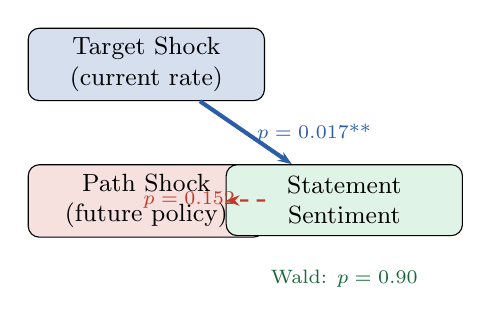
\begin{tikzpicture}[
  box/.style={draw, rounded corners, minimum width=3cm, minimum height=0.9cm,
    font=\small, align=center},
  arr/.style={-{Stealth[length=5pt]}, thick}
]
\node[box, fill=myblue!20] (target) {Target Shock\\(current rate)};
\node[box, fill=myred!15, below=0.8cm of target] (path) {Path Shock\\(future policy)};
\node[box, fill=mygreen!15, below right=0.8cm and -0.5cm of target] (sent) {Statement\\Sentiment};

\draw[arr, myblue, line width=1.5pt] (target) -- node[right, font=\scriptsize]{$p=0.017$**} (sent);
\draw[arr, myred, line width=0.8pt, dashed] (path) -- node[left, font=\scriptsize]{$p=0.152$} (sent);

\node[font=\scriptsize, text=mygreen!60!black, below=0.3cm of sent] {Wald: $p=0.90$};
\end{tikzpicture}
\par\vspace{0.15em}
{\scriptsize \textbf{Figure 2.} Implementation vs.\ Revelation}
\end{center}
\end{columns}
\end{frame}

% ============================================================
\begin{frame}{Forward Guidance Does Not Strengthen the Language Channel}
\begin{center}
{\small \textbf{Table 4.} Forward Guidance Period Interaction (H4)}
\end{center}
\vspace{0.1em}
\begin{center}
{\small
\begin{tabular}{lcc}
\toprule
Variable & CRSP VW & NASDAQ \\
\midrule
Target shock & $-0.421$ & $-0.289$ \\
 & $(0.046)$ & $(0.031)$ \\
Path shock & $-0.175$ & $-0.166$ \\
 & $(0.452)$ & $(0.320)$ \\
Sentiment & $-20.73$ & $5.47$ \\
 & $(0.191)$ & $(0.709)$ \\
\textbf{Sentiment $\times$ FG} & $-3.72$ & $6.04$ \\
 & $\mathbf{(0.836)}$ & $\mathbf{(0.739)}$ \\
\midrule
$R^2$ & 9.9\% & 3.5\% \\
\bottomrule
\end{tabular}
}
\end{center}

\vspace{0.2em}
\begin{aalertblock}{Result}
Interaction \textbf{not significant} --- sentiment does not become more important during FG period
\end{aalertblock}
\end{frame}

% ============================================================
\section{Robustness}
% ============================================================

\begin{frame}{Results Robust Across Sentiment Measures and Documents}
\begin{center}
{\small \textbf{Table 5.} Alternative Sentiment Measures}
\end{center}
\vspace{0.1em}
\begin{center}
{\footnotesize
\begin{tabular}{lccccc}
\toprule
Model & $\beta_T$ & $p_T$ & $\beta_P$ & $p_P$ & $R^2$ \\
\midrule
Statement Comb. & 0.000577** & 0.017 & 0.000633 & 0.152 & 1.57\% \\
Minutes LM & 0.000918* & 0.083 & 0.001091 & 0.324 & 3.67\% \\
Minutes CB & 0.000147 & 0.716 & 0.001423* & 0.061 & 5.60\% \\
\textbf{Minutes Comb.} & \textbf{0.000532**} & \textbf{0.011} & \textbf{0.001257**} & \textbf{0.015} & \textbf{9.35\%} \\
Statement + Min. & 0.000391* & 0.062 & 0.000194 & 0.611 & 6.06\% \\
\bottomrule
\end{tabular}
}
\end{center}

\vspace{0.2em}
\begin{columns}[T]
\column{0.48\textwidth}
\begin{aexampleblock}{CB Outperforms LM}
CB captures hawkish/dovish language that LM misses
\end{aexampleblock}

\column{0.48\textwidth}
\begin{ablock}{Minutes Reveal Path Info}
Path shock significant ($p = 0.015$) in Minutes
\end{ablock}
\end{columns}
\end{frame}

% ============================================================
\begin{frame}{Robustness: Standard Errors, COVID, Regimes}
\begin{columns}[T]
\column{0.48\textwidth}
\begin{ablock}{Alternative SE \& Lags}
\begin{itemize}
  \item NW HAC(2), HAC(4), HAC(6)
  \item White heteroskedasticity-robust
  \item Target significant across all
  \item Path insignificant across all
\end{itemize}
\end{ablock}
\vspace{0.2em}
\begin{aexampleblock}{Excluding COVID}
\begin{itemize}
  \item Results unchanged
  \item Target: $p \approx 0.02$
  \item Path: $p \approx 0.16$
\end{itemize}
\end{aexampleblock}

\column{0.48\textwidth}
\begin{ablock}{Regime Heterogeneity}
\begin{itemize}
  \item \textbf{FG} ($N\!=\!61$): Target $p\!<\!0.001$
  \item \textbf{Norm.} ($N\!=\!49$): Neither significant
  \item \textbf{Conv.} ($N\!=\!7$): Too few obs.
\end{itemize}
\end{ablock}
\vspace{0.2em}
\begin{aalertblock}{Bauer-Swanson (2023)}
Shocks partially predictable ($R^2 \approx 11$--$14\%$), but critique applies to \emph{both} target and path
\end{aalertblock}
\end{columns}
\end{frame}

% ============================================================
\begin{frame}{Extension: JK Sign-Restriction Decomposition}
\begin{columns}[T]
\column{0.48\textwidth}
\begin{ablock}{Method (Jarociński \& Karadi 2020)}
Classify target shocks by sign restriction:
\begin{itemize}
  \item \textbf{MP shock}: rate $\uparrow$, stocks $\downarrow$ (59\%)
  \item \textbf{CBI shock}: rate $\uparrow$, stocks $\uparrow$ (41\%)
\end{itemize}
\vspace{0.2em}
{\small CBI = central bank information effect}
\end{ablock}

\column{0.48\textwidth}
\begin{ablock}{H1: Sentiment Regression}
{\small
\begin{tabular}{lcc}
\toprule
 & Coeff. & $p$ \\
\midrule
$\beta_\text{MP}$ & 0.000541 & 0.134 \\
$\beta_\text{CBI}$ & 0.000653 & 0.170 \\
$\beta_P$ & 0.000643 & 0.159 \\
\midrule
$R^2$ & \multicolumn{2}{c}{1.58\%} \\
\bottomrule
\end{tabular}
}
\end{ablock}
\end{columns}

\vspace{0.3em}
\begin{aalertblock}{Key Finding}
Neither MP nor CBI component significant for sentiment; F-test cannot reject $\beta_\text{MP} = \beta_\text{CBI}$ ($p = 0.87$). Decomposition loses significance due to reduced power in subgroups.
\end{aalertblock}
\end{frame}

% ============================================================
\begin{frame}{Extension: JK Decomposition — Asset Returns}
\begin{columns}[T]
\column{0.48\textwidth}
\begin{ablock}{H2: CRSP VW Returns}
{\small
\begin{tabular}{lcc}
\toprule
 & Coeff. & $p$ \\
\midrule
$\beta_\text{MP}$ & $-1.029$ & $<0.001$*** \\
$\beta_\text{CBI}$ & $0.844$ & $<0.001$*** \\
$\beta_P$ & $-0.019$ & 0.911 \\
\midrule
$R^2$ & \multicolumn{2}{c}{35.69\%} \\
\bottomrule
\end{tabular}
}
\end{ablock}

\column{0.48\textwidth}
\begin{aexampleblock}{Interpretation}
\begin{itemize}
  \item \textbf{MP shocks}: contractionary $\to$ stocks fall ($\beta = -1.03$***)
  \item \textbf{CBI shocks}: rate hike + stocks rise $\to$ information effect ($\beta = +0.84$***)
  \item \textbf{Path shock}: still insignificant
  \item R$^2$ jumps from 9.1\% to 35.7\%
\end{itemize}
\end{aexampleblock}
\end{columns}

\vspace{0.3em}
\begin{center}
{\small JK decomposition \textbf{confirms} the information effect in asset markets, but sentiment does not differentiate MP from CBI}
\end{center}
\end{frame}

% ============================================================
\begin{frame}{Extension: Bauer-Swanson Orthogonalization}
\begin{columns}[T]
\column{0.48\textwidth}
\begin{ablock}{Method}
Regress shocks on pre-FOMC macro info, use residuals:
\begin{itemize}
  \item Target predictability: $R^2 = 10.5\%$
  \item Path predictability: $R^2 = 13.8\%$
\end{itemize}
\vspace{0.2em}
{\small Controls: lagged returns, VIX, term spread, rate changes}
\end{ablock}

\column{0.48\textwidth}
\begin{ablock}{H1: Sentiment (Orthogonalized)}
{\small
\begin{tabular}{lcc}
\toprule
 & Original & Orthogonalized \\
\midrule
$\beta_T$ & 0.000592** & 0.000631 \\
 & (0.012) & (0.108) \\
$\beta_P$ & 0.000666 & $-0.000963$ \\
 & (0.131) & (0.193) \\
\midrule
$R^2$ & 1.70\% & 2.00\% \\
\bottomrule
\end{tabular}
}
\end{ablock}
\end{columns}

\vspace{0.3em}
\begin{aalertblock}{Key Finding}
Target loses significance ($p = 0.012 \to 0.108$) after B-S orthogonalization, but path remains insignificant. For asset returns, target \textbf{strengthens} ($p = 0.043 \to 0.005$).
\end{aalertblock}
\end{frame}

% ============================================================
\section{Conclusion}
% ============================================================

\begin{frame}{Summary of Findings}
\begin{columns}[T]
\column{0.48\textwidth}
\begin{ablock}{What We Find}
\begin{enumerate}
  \item Target shock \textbf{significantly} predicts statement sentiment ($p = 0.017$)
  \item Path shock does \textbf{not} ($p = 0.152$)
  \item Target shock drives equity responses; path effects are weak
  \item EW $>$ VW: financing-channel evidence
  \item FG interaction \textbf{not significant}
  \item CB dictionary outperforms LM
  \item Minutes reveal path information
\end{enumerate}
\end{ablock}

\column{0.48\textwidth}
\begin{aalertblock}{What We Cannot Claim}
\begin{itemize}
  \item Wald test cannot reject $\beta_T = \beta_P$ ($p = 0.90$)
  \item $R^2$ is modest (1.57\%)
  \item Cannot fully separate communication from policy effects
  \item Daily frequency may miss intraday channels
\end{itemize}
\end{aalertblock}
\vspace{0.2em}
\begin{aexampleblock}{Bottom Line}
Evidence \textbf{favors} implementation over revelation, but cannot eliminate information effects
\end{aexampleblock}
\end{columns}
\end{frame}

% ============================================================
\begin{frame}{Relation to Fernández-Fuertes (2025)}
\begin{columns}[T]
\column{0.48\textwidth}
\begin{fblock}[5.5cm]{FF: Better Shock Measure}
\begin{itemize}
  \item Multi-agent LLM $\to$ narrative surprises
  \item Processes Statements, Minutes, Beige Books, Press Conferences
  \item His Table 32: target $\beta_T = 0.047^{***}$, path $\beta_P \approx 0$
  \item \textbf{Same target-dominant pattern}
  \item R$^2$ = 12.4\% vs.\ our 1.57\%
\end{itemize}
\end{fblock}

\column{0.48\textwidth}
\begin{falertblock}[5.5cm]{Us: What Does Language Convey?}
\begin{itemize}
  \item Different question, not different method
  \item 4 structured hypotheses + Wald + FG interaction
  \item Statement vs.\ Minutes channel comparison
  \item Fully transparent \& reproducible
  \item No API dependencies
\end{itemize}
\end{falertblock}
\end{columns}

\vspace{0.3em}
\begin{center}
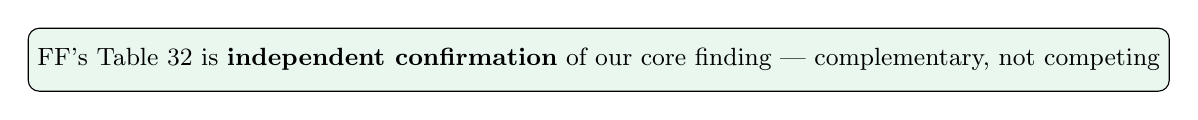
\begin{tikzpicture}
\node[draw, rounded corners, fill=mygreen!10, minimum width=12cm, minimum height=0.8cm, font=\small] {
FF's Table 32 is \textbf{independent confirmation} of our core finding --- complementary, not competing
};
\end{tikzpicture}
\end{center}
\end{frame}

% ============================================================
\begin{frame}{Future Directions}
\begin{columns}[T]
\column{0.48\textwidth}
\begin{ablock}{Methodological Extensions}
\begin{itemize}
  \item LLM-based sentiment (Chen et al.\ 2025; FF 2025)
  \item Bauer-Swanson orthogonalized shocks
  \item Intraday event windows (TAQ data)
  \item JK (2020) info vs.\ monetary decomposition
\end{itemize}
\end{ablock}

\column{0.48\textwidth}
\begin{ablock}{Data Extensions}
\begin{itemize}
  \item Extend GSS series to 2025 (USMPD)
  \item Press conference transcripts
  \item SEP projections and dot plots
  \item Cross-country central bank communication
\end{itemize}
\end{ablock}
\end{columns}

\vspace{0.5em}
\begin{center}
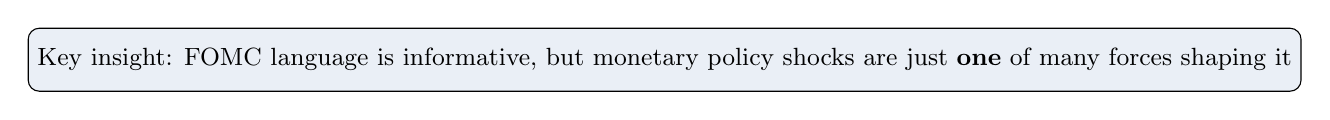
\begin{tikzpicture}
\node[draw, rounded corners, fill=myblue!10, minimum width=10cm, minimum height=0.8cm, font=\small] {
Key insight: FOMC language is informative, but monetary policy shocks are just \textbf{one} of many forces shaping it
};
\end{tikzpicture}
\end{center}
\end{frame}

% ============================================================
\begin{frame}[plain]
\begin{center}
\vspace{2cm}
{\LARGE\bfseries Thank You}\\[1em]
{\large Questions \& Discussion}\\[2em]
{\small Eileen Zhang \quad Dechang Yang}\\[0.3em]
{\small Xi'an Jiaotong-Liverpool University}\\[0.5em]
{\footnotesize Words Beyond the Rate: High-Frequency Monetary Policy Shocks and FOMC Language}
\end{center}
\end{frame}

\end{document}
